\documentclass[a4paper,11pt]{article}

\usepackage[english]{babel}
\usepackage[utf8]{inputenc}
\usepackage[vmargin=3.5cm,hmargin=2cm]{geometry}
\usepackage{graphicx}
\usepackage{caption}
\usepackage{subcaption}
\usepackage{amsmath}
\usepackage{mathtools}
\usepackage{fancyhdr}
\usepackage{listings}

\setlength{\footskip}{0cm}
\setlength\parindent{0pt}
\addtolength{\footskip}{0.8cm}
\addtolength{\headsep}{-.5cm}

\title{\bfseries Lab 6.1: \\ Linear Modulation with Two-dimensional Constellations\\}
\date{}

\lfoot{}
\cfoot{}
\rfoot{\textbf{Communication Systems} \\ Teresa Algarra Ulierte }

\renewcommand{\headrulewidth}{0.5pt}
\renewcommand{\footrulewidth}{0.5pt}

\begin{document}
\renewcommand\contentsname{\vspace{-1cm}}
\maketitle
\lstset{language=Matlab}

\begin{centering}
    Teresa Algarra Ulierte \\
    Student ID: teresaalgarraulierte \\
    Perm number: 7626872 \\
\end{centering}

\vspace{3cm}

\begin{figure}[!ht]
	\centering
	
\includegraphics[scale = 5]{images/portada.jpeg}
\end{figure}

\newpage

\section{Goal of the lab:}

This is a follow-on to Software Lab 4.1, the code from which is the starting
point here. The objective was to implement in complex baseband a linearly
modulated system for a variety of signal constellations. I estimated the
performance of these schemes for an ideal channel via simulation, and compared
them with analytical expressions.

\section{Laboratory assignment:}

The first step was to write a MatLab function that would generate random bits
taking values in ${0,1}$ with equal probability. It was done with the function
\textbf{randi} and needing only the desired length as input.

\bigskip
\begin{lstlisting}

  function [r] = randbit(len_in)
      r = randi([0,1],len_in,1);
  end

\end{lstlisting}
\bigskip

For the rest of the lab, I worked with five different constellations: BPSK,
QPSK, 4PAM, 16QAM and 8PSK.

\subsection{BPSK}

To map bits from the vector generated by \textbf{randbit} I created a script
that maps $0$ to $-1$ and $+1$ to $+1$:

\bigskip
\begin{lstlisting}

function [y] = bpskmap(x)
    len = length(x);
    y = zeros(1,len);

    for i = 1:len
        if x(i) == 0
            y(i) = -1;
        elseif x(i) == 1
            y(i) = 1;
        end
    end
end

\end{lstlisting}
\bigskip

I created a 12000-long bit string and mapped it to BPSK. Using the code from
\textit{Lab 4.1}, I passed it through the transmit filter, that it, upsampled
it and convoluted it with the SRRC pulse. Then, I added noise to the channel
by calculating the $SNR$ with the Q function (the result was 2.71 to get a 1%
error) and getting $N_0$ from there doing $N_0 = \displaystyle\frac{E_b}{SNR}$.
Then I passed it through the receive filter, that is, convoluted it with the
SRRC pulse again and downsampled it. Then I mapped inversely the constellation
back to ${0,1}$ bits with the following script:

\bigskip
\begin{lstlisting}

function [y] = bpskmapinverse(x)
    len = length(x);
    y = zeros(1,len);

    for i = 1:len
        if real(x(i)) < 0
            y(i) = 0;
        elseif real(x(i)) > 0
            y(i) = 1;
        end
    end
end

\end{lstlisting}
\bigskip

The error resulting of this whole process is approximately $1.005$ (it varies
slightly with every operation).

In this plot we can clearly see the comparison between the noiseless mapped
signal and the signal at the output of the receive filter after the noise had
been added:

\begin{figure}[!hp]
    \begin{center}
      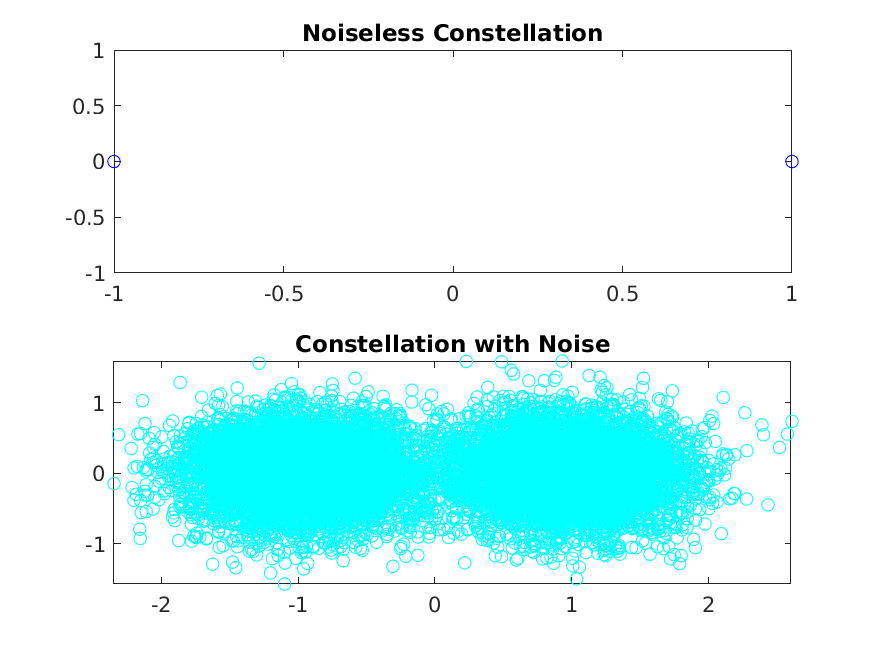
\includegraphics[width=1\textwidth]{images/BPSK.png}
      \captionof{figure}{BPSK}
    \end{center}
\end{figure}

\newpage

\subsection{4PAM}

For the 4PAM constellation the process was the same. To map the bits to 4PAM,
the code used took two vectors and outputed one:

\bigskip
\begin{lstlisting}

function [y] = fourpammap(x1, x2)
    len = length(x1);
    y = zeros(1,len);

    for i = 1:len
        bits = [x1(i),x2(i)];
        if bits == [0,0]
            y(i) = -3;
        elseif bits == [0,1]
            y(i) = -1;
        elseif bits == [1,0]
            y(i) = +1;
        elseif bits == [1,1]
            y(i) = +3;
        end
    end
end

\end{lstlisting}
\bigskip

The noise value was different, being the SNR of 2.71. The code to reverse the
mapping process was:

\bigskip
\begin{lstlisting}

function [y1, y2] = fourpammapinverse(x)
    len = length(x);
    y1 = zeros(1,len);
    y2 = zeros(1,len);

    for i = 1:len
        if (x(i) <= -2)
            y1(i) = 0;
            y2(i) = 0;
        elseif (x(i) > -2) && (x(i) <= 0)
            y1(i) = 0;
            y2(i) = 1;
        elseif (x(i) > 0) && (x(i) <= 2)
            y1(i) = 1;
            y2(i) = 0;
        elseif (x(i) > 2)
            y1(i) = 1;
            y2(i) = 1;
        end
    end
end

\end{lstlisting}
\bigskip

The resulting error was around 1 too, varying with every iteration.

In this plot we can clearly see the comparison between the noiseless mapped
signal and the signal at the output of the receive filter after the noise had
been added:

\begin{figure}[!hp]
    \begin{center}
      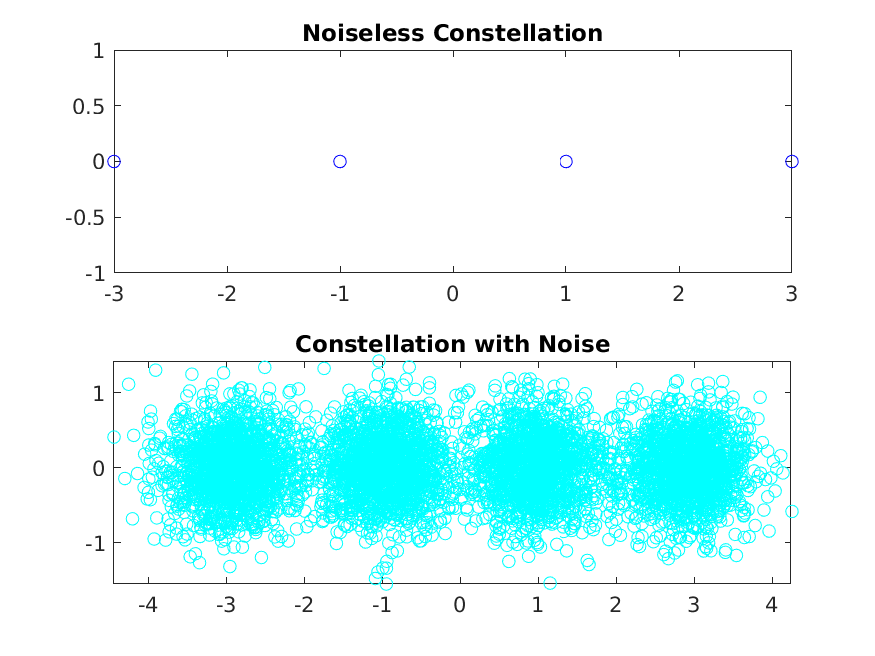
\includegraphics[width=1\textwidth]{images/4PAM.png}
      \captionof{figure}{4PAM}
    \end{center}
\end{figure}

\newpage

\subsection{QPSK}

For QPSK the process and the noise values were the same as for 4PAM. The code
to map from bits to BPSK took two vectors as input, and followed the scheme:

\bigskip
\begin{lstlisting}

  if bits == [0,0]
      y(i) = -1 -1j;
  elseif bits == [0,1]
      y(i) = -1 +1j;

\end{lstlisting}
\bigskip

To reverse the process, the code followed the pattern:

\bigskip
\begin{lstlisting}

  if (real(x(i))<=0) &&  (imag(x(i))<=0)
    y1(i) = 0;
    y2(i) = 0;
  elseif (real(x(i))<=0) &&  (imag(x(i))>0)
    y1(i) = 0;
    y2(i) = 1;

\end{lstlisting}
\bigskip

The resulting error was, once again, around 1, varying slightly every iteration.

In this plot we can clearly see the comparison between the noiseless mapped
signal and the signal at the output of the receive filter after the noise had
been added:

\begin{figure}[!hp]
    \begin{center}
      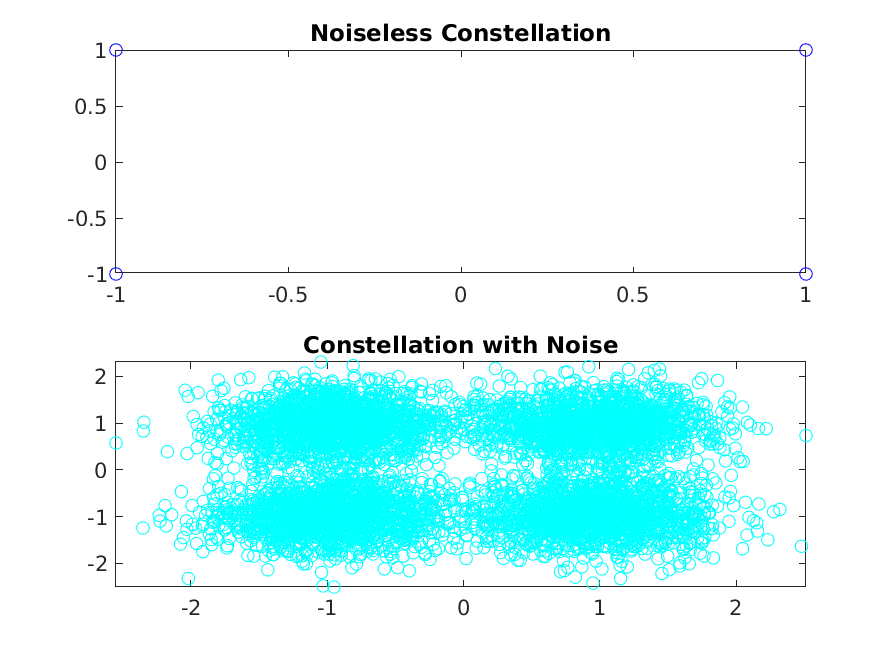
\includegraphics[width=0.7\textwidth]{images/QPSK.png}
      \captionof{figure}{QPSK}
    \end{center}
\end{figure}

\newpage

\subsection{16QAM}

For 16QAM the process and the noise values were the same as for 4PAM. The code
to map from bits to 16QAM took four vectors as input, and followed the scheme:

\bigskip
\begin{lstlisting}

  if bits == [0,0,0,0]
      y(i) = -3 -3j;
  elseif bits == [0,0,0,1]
      y(i) = -3 -1j;

\end{lstlisting}
\bigskip

To reverse the process, the code followed the pattern:

\bigskip
\begin{lstlisting}

  if (real(x(i))<=-2)&&(imag(x(i))<=-2)
      y1(i) = 0;
      y2(i) = 0;
      y3(i) = 0;
      y4(i) = 0;
  elseif (real(x(i))<=-2)&&(imag(x(i))>-2)&&(imag(x(i))<=0)
      y1(i) = 0;
      y2(i) = 0;
      y3(i) = 0;
      y4(i) = 1;

\end{lstlisting}
\bigskip

The resulting error was, once again, around 1, varying slightly every iteration.

In this plot we can clearly see the comparison between the noiseless mapped
signal and the signal at the output of the receive filter after the noise had
been added:

\begin{figure}[!hp]
    \begin{center}
      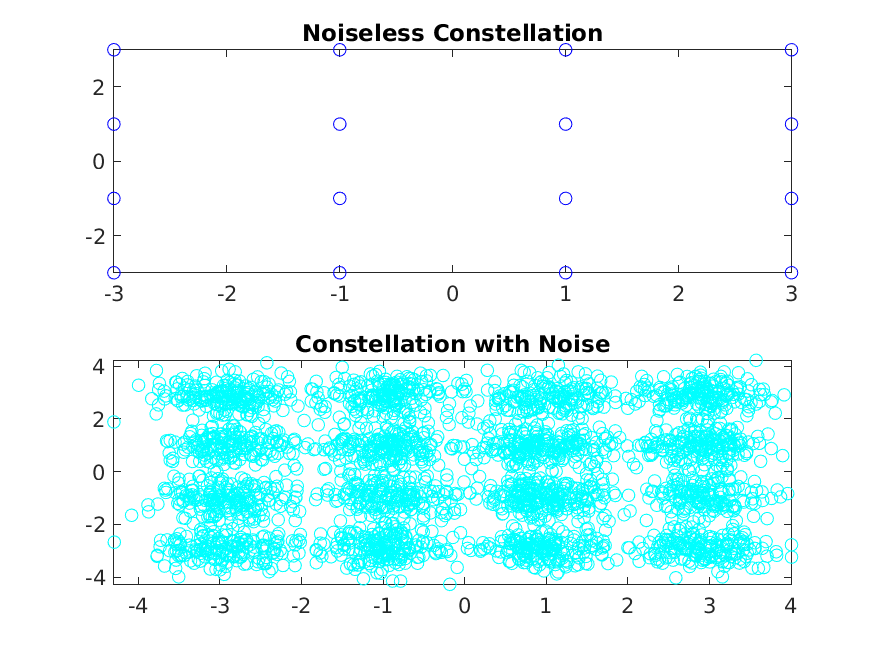
\includegraphics[width=0.55\textwidth]{images/16QAM1.png}
      \captionof{figure}{16QAM}
    \end{center}
\end{figure}

\newpage

\subsection{8PSK}

Lastly, for 8PSK the noise was calculated differently, being the $SNR$ 6.16.
The mapping code included exponentials as shown:

\bigskip
\begin{lstlisting}

  if bits == [0,0,0]
      y(i) = exp(0*1j*2*pi/8);
  elseif bits == [0,0,1]
      y(i) = exp(1*1j*2*pi/8);

\end{lstlisting}
\bigskip

To reverse the process, the code followed the pattern:

\bigskip
\begin{lstlisting}

  if (angle(x(i))>=-pi/8)&&(angle(x(i))<=pi/8)
    y1(i) = 0;
    y2(i) = 0;
    y3(i) = 0;
  elseif (angle(x(i))>pi/8)&&(angle(x(i))<=3*pi/8)
    y1(i) = 0;
    y2(i) = 0;
    y3(i) = 1;

\end{lstlisting}
\bigskip

The error was, as expected, around 1 for every iteration.

In this plot we can clearly see the comparison between the noiseless mapped
signal and the signal at the output of the receive filter after the noise had
been added:

\begin{figure}[!hp]
    \begin{center}
      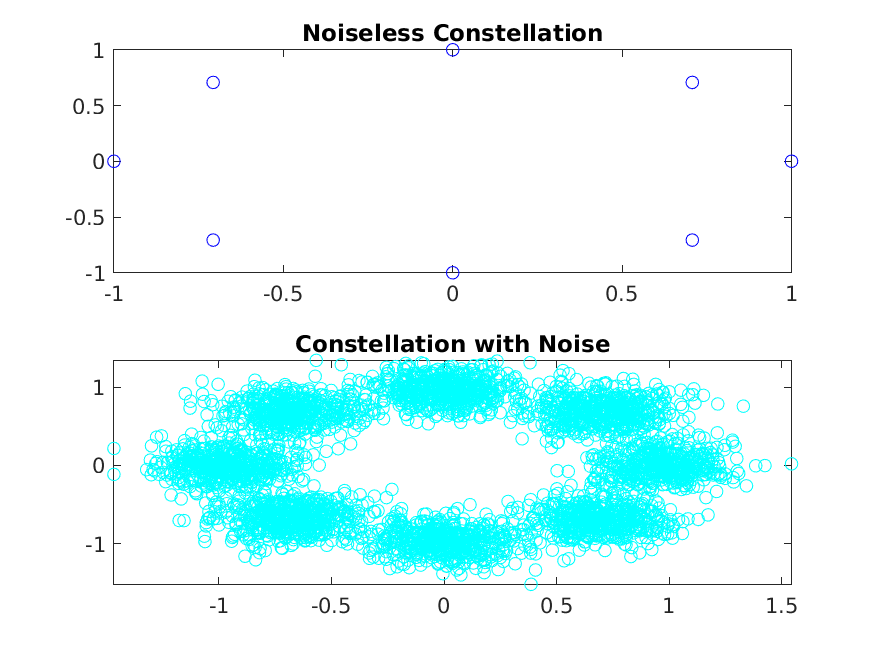
\includegraphics[width=0.6\textwidth]{images/8PSK.png}
      \captionof{figure}{8PSK}
    \end{center}
\end{figure}

\newpage


\subsection{16QAM with no ISI}

For this last step, the code was simplified by eliminating the upsampling,
convolution with transmit filter, convolution with receive filter and
downsampling. Therefore, the noise was added directly to the mapped 16QAM
vector and decoded right after. The functions used were the same as for the
regular 16QAM section. Using the same noise data as before the error did not
vary significantly, it was still around 1%:

\begin{figure}[!hp]
    \begin{center}
      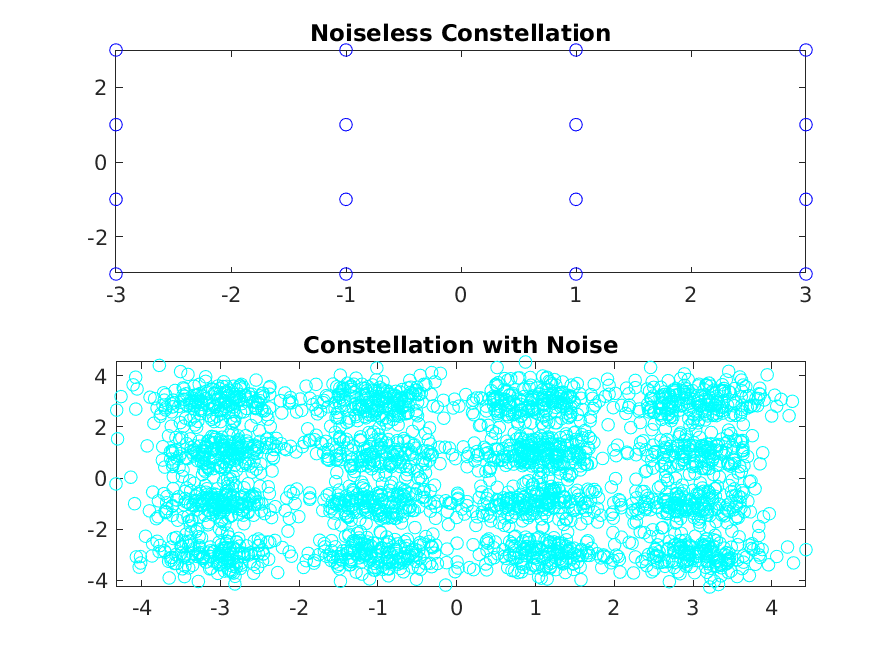
\includegraphics[width=0.55\textwidth]{images/16QAM2.png}
      \captionof{figure}{16QAM with the same noise}
    \end{center}
\end{figure}

Nevertheless, when using $3dB$ more for the SNR, the error percentage
dropped to 0.25%, even though it is hard to appreciate in the plot:

\begin{figure}[!hp]
    \begin{center}
      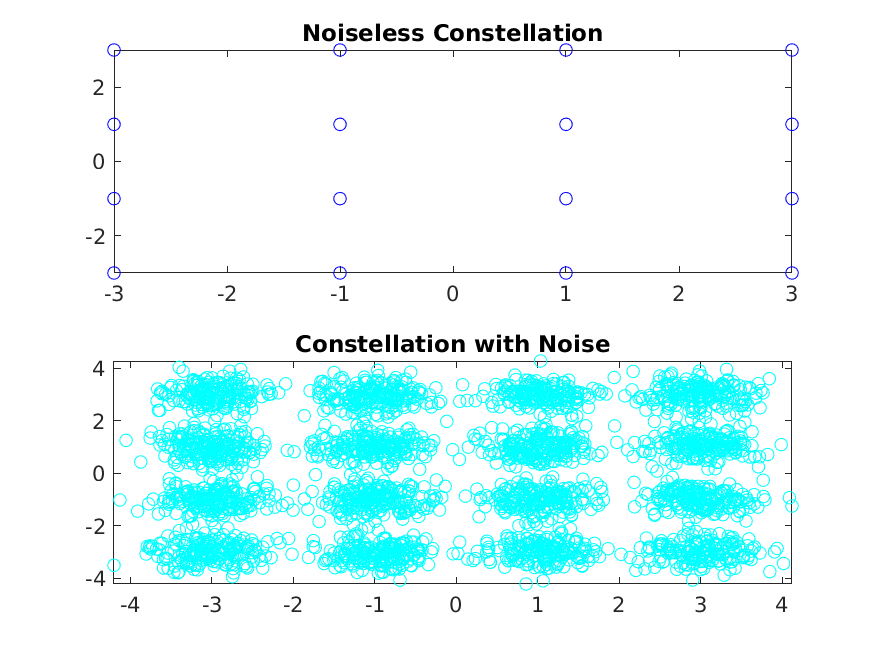
\includegraphics[width=0.55\textwidth]{images/16QAM3.png}
      \captionof{figure}{16QAM with 3dB more SNR}
    \end{center}
\end{figure}

\newpage

\section{Conclusion:}

This lab was an useful continuation to Lab 4.1. There I learnt how to use
constellations and how to visualize them, whereas with Lab 6.1 I learnt how
to code each one of them, as well as to compare them with one another.
It was also very helpful to understand how the error in a transmission channel
happens and how to calculate it.

I had to be very careful and systematic to be able to write correctly the
scripts to map and reverse the mapping process, specially for 16QAM and
8PSK, since those were the longest and more complex ones.

Overall, it was a not excessively long lab and not too hard, but complex enough
to make me think about everything twice and to help me understand the theory
seen in class through actual plots and error percentages.

\vspace{4cm}

\end{document}
